%!TEX root = Slic3r-Manual.tex

\section{L'impression} % (fold)
\label{sec:printing}
\index{Printing}
\index{impression}

A ce stade Slic3r est configur\'e et un mod\`ele 3D a \'et\'e obtenu, converti et pr\^et \`a l'emploi pour l'impression. Maintenant il est temps de d\'emarrer l'imprimante et de l'essayer.

Une vari\'et\'e de logiciels est disponible pour envoyer le code G \`a l'imprimante. Voici quelques solutions open-source: Printrun\footnote{\url{https://github.com/kliment/Printrun}}, Repetier\footnote{\url{http://www.repetier.com/}} et Repsnapper\footnote{\url{https://github.com/timschmidt/repsnapper}}.

Pour les imprimantes \'equip\'ee d'un lecteur de carte m\'emoire et d'un panneau de commande, le ficher G-code produit par Slic3r peut \^etre interpr\'et\'e par l'imprimante, depuis la carte m\'emoire.
\begin{figure}[H]
\centering
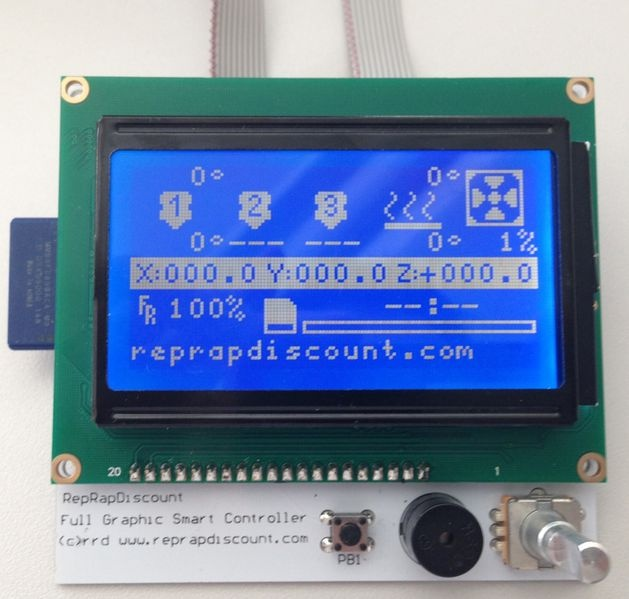
\includegraphics[keepaspectratio=true,width=0.5\textwidth]{printing/glcd.jpg}
\caption{Un mod\`ele de panneau de commande}
\label{fig:glcd}
\end{figure}
Les sections suivantes porteront sur les param\`etres disponibles en mode simple et mode expert, et sur l'etude des techniques d'impression avanc\'ees, y compris des cas particuliers ainsi que le d\'epannage.

% section first_print (end)